\documentclass[a4paper,11pt]{article}
\pdfoutput=1

\usepackage{jinstpub}
\usepackage{siunitx}
\sisetup{range-phrase=--, range-units=single, separate-uncertainty=true}

% Draft notes for Dylan: remove (or \renewcommand to empty) before submission.
\usepackage{xcolor}
\newcommand{\askDylan}[1]{\textcolor{cyan!60!black}{[\textbf{Dylan:} #1]}}

\title{\boldmath Searching for X17 at n\_TOF with large-area Micromegas detectors in $\mu$TPC mode}

\author[a,1]{D.~Neff\note{Corresponding author.}}
\affiliation[a]{AFFILIATION,\\ADDRESS, COUNTRY} % TODO Dylan
\emailAdd{name@example.org} % TODO Dylan

\collaboration{on behalf of the n\_TOF Collaboration} % TODO Dylan: confirm wording and co-author list

\abstract{%
The ATOMKI anomaly in the angular correlation of $e^+e^-$ pairs from nuclear transitions has been
interpreted as a new boson of mass $\approx\SI{17}{MeV}$, X17. An independent search in the
$^3$He$(n,e^+e^-)^4$He channel was carried out at the n\_TOF EAR2 facility at CERN in July and August 2026,
using four large-area ($40\times\SI{40}{cm^2}$) resistive-strip bulk Micromegas operated as
micro-TPCs to measure the opening angle of the pair. We describe the detectors and a waveform
forward-model reconstruction that accounts for the delayed charge sharing between resistive strips,
which biases per-strip hit times. On a cosmic-ray bench the best chamber reconstructs 93\% of
reference muons within \SI{5}{mm}, with a per-plane angular resolution of about \ang{1.2}, and a
spatial resolution of \SI{176}{\micro m} was measured in a beam. At n\_TOF the $\gamma$ flash
saturates the DREAM front end for milliseconds while the chambers themselves recover within
microseconds; the recorded data therefore cover the thermal-neutron window. The campaign recorded
\num{41.8e6} events, and first reconstructed tracks from opposing chambers point back to the
$^3$He target.}

\keywords{Micropattern gaseous detectors (MSGC, GEM, THGEM, RETHGEM, MHSP, MICROPIC, MICROMEGAS, InGrid, etc.);
Time projection Chambers (TPC); Front-end electronics for detector readout}

\proceeding{9$^{\text{th}}$ International Conference on Micro Pattern Gaseous Detectors (MPGD2026)\\
  30 August -- 4 September 2026\\
  Prague, Czech Republic}

\notoc

\begin{document}
\maketitle
\flushbottom

%% ------------------------------------------------------------------------------------------
\section{Introduction}
\label{sec:intro}

The ATOMKI group reported an excess of $e^+e^-$ pairs at large opening angles in the decay of
excited states of $^8$Be~\cite{Krasznahorkay2016}, $^4$He~\cite{Krasznahorkay2021} and
$^{12}$C~\cite{Krasznahorkay2022}, consistent with the emission of a neutral boson of mass
$\approx\SI{16.8}{MeV}$ decaying to $e^+e^-$ (X17). The $^4$He case can be reached independently with
neutrons: capture on $^3$He forms $^4$He$^*$ \SI{20.58}{MeV} above the ground state, which
de-excites by $\gamma$ emission, by internal pair creation (IPC) or, possibly, by X17
emission~\cite{Viviani2022}. A massive X17 is produced nearly at rest, so its decay pair is emitted
almost back to back (opening angle above \ang{109} for any decay orientation), whereas the IPC
pairs peak at small angles. The observable is therefore the opening-angle spectrum of $e^+e^-$
pairs from a $^3$He target, which must be measured before the leptons scatter in any material.

This contribution describes the large-area Micromegas $\mu$TPCs built for that measurement, their
reconstruction and performance, and the 2026 campaign at the n\_TOF EAR2 facility, with emphasis on
the experience of operating MPGDs in its $\gamma$ flash.

%% ------------------------------------------------------------------------------------------
\section{The MX17 Micromegas $\mu$TPC}
\label{sec:detector}

The MX17 chambers (figure~\ref{fig:detector}, left) were designed and built at CEA Saclay. Each is a
resistive-strip bulk Micromegas~\cite{Giomataris1996,Alexopoulos2011} with a \SI{30}{mm} drift gap
and a \SI{150}{\micro m} amplification gap, read out over an active area of about
$40\times\SI{36}{cm^2}$. The resistive strips (\SI{0.80}{mm} pitch) are capacitively coupled to a
$512\times512$ matrix of square pads (\SI{0.68}{mm} on a \SI{0.78}{mm} pitch), each pad routed to an
$x$ or a $y$ strip on lower layers, giving two orthogonal views of 512 channels each. Every chamber
is read out by two DREAM front-end units~\cite{DREAM} (1024 channels), which sample each strip's
shaped signal every \SI{20}{ns}.

In $\mu$TPC mode the arrival time of the ionisation at the mesh gives its drift depth. For a
track inclined by $\theta$ in one view, the transverse position $x$ and depth $z$ of each strip's
charge give $\tan\theta = \mathrm{d}x/\mathrm{d}z$. On a resistive anode, however, a fraction of the
charge reaches the neighbouring strips through the resistive layer, \emph{delayed and dispersed} by
its RC time constant~\cite{Dixit2004,Galan2012}. The resulting signal on each strip is the
superposition of its own charge and late copies of its neighbours'. Measured with cosmic muons, the
first neighbour receives about 5\% of the charge in the view whose strips run across the resistive
strips and about 15\% in the view along them (figure~\ref{fig:detector}, right). Any per-strip time
estimator (threshold crossing, constant fraction or matched filter) is pulled late on the edges of
the cluster: the reconstructed drift-time ladder is compressed by 20--30\% and the angle reads
about \ang{4} too steep.

\begin{figure}[htbp]
\centering
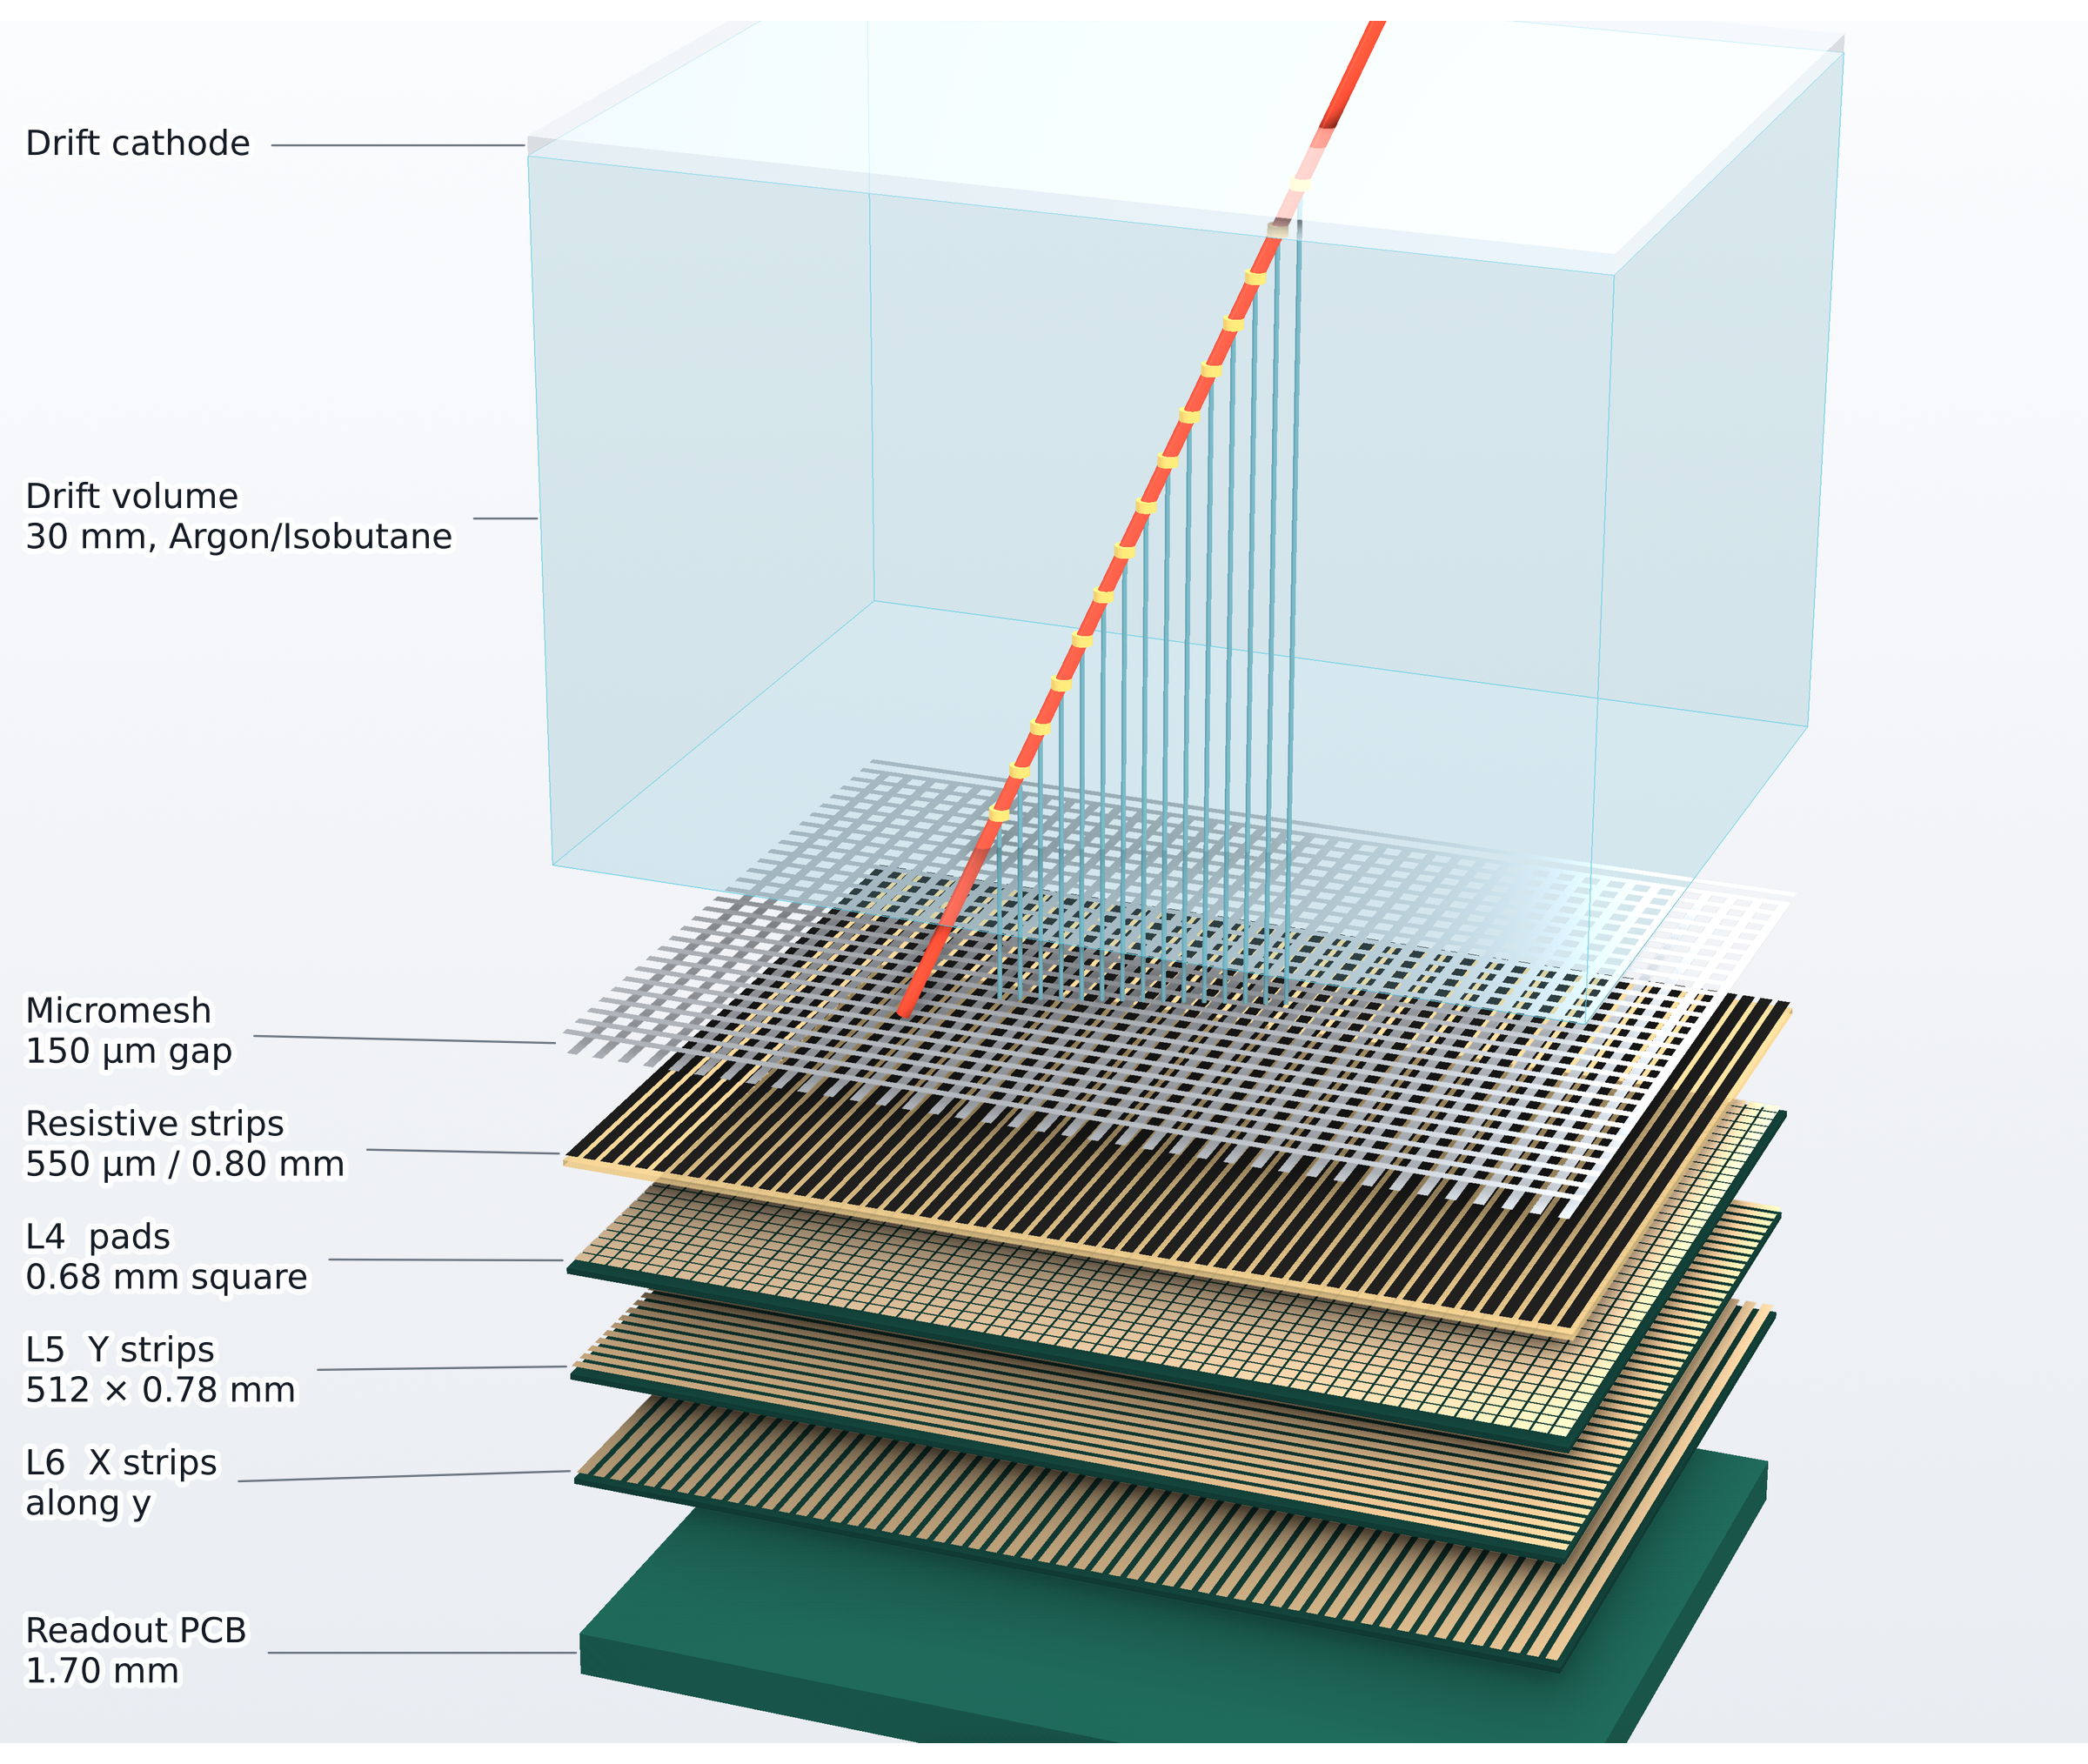
\includegraphics[width=0.44\textwidth]{figures/chamber_exploded.png}
\hfill
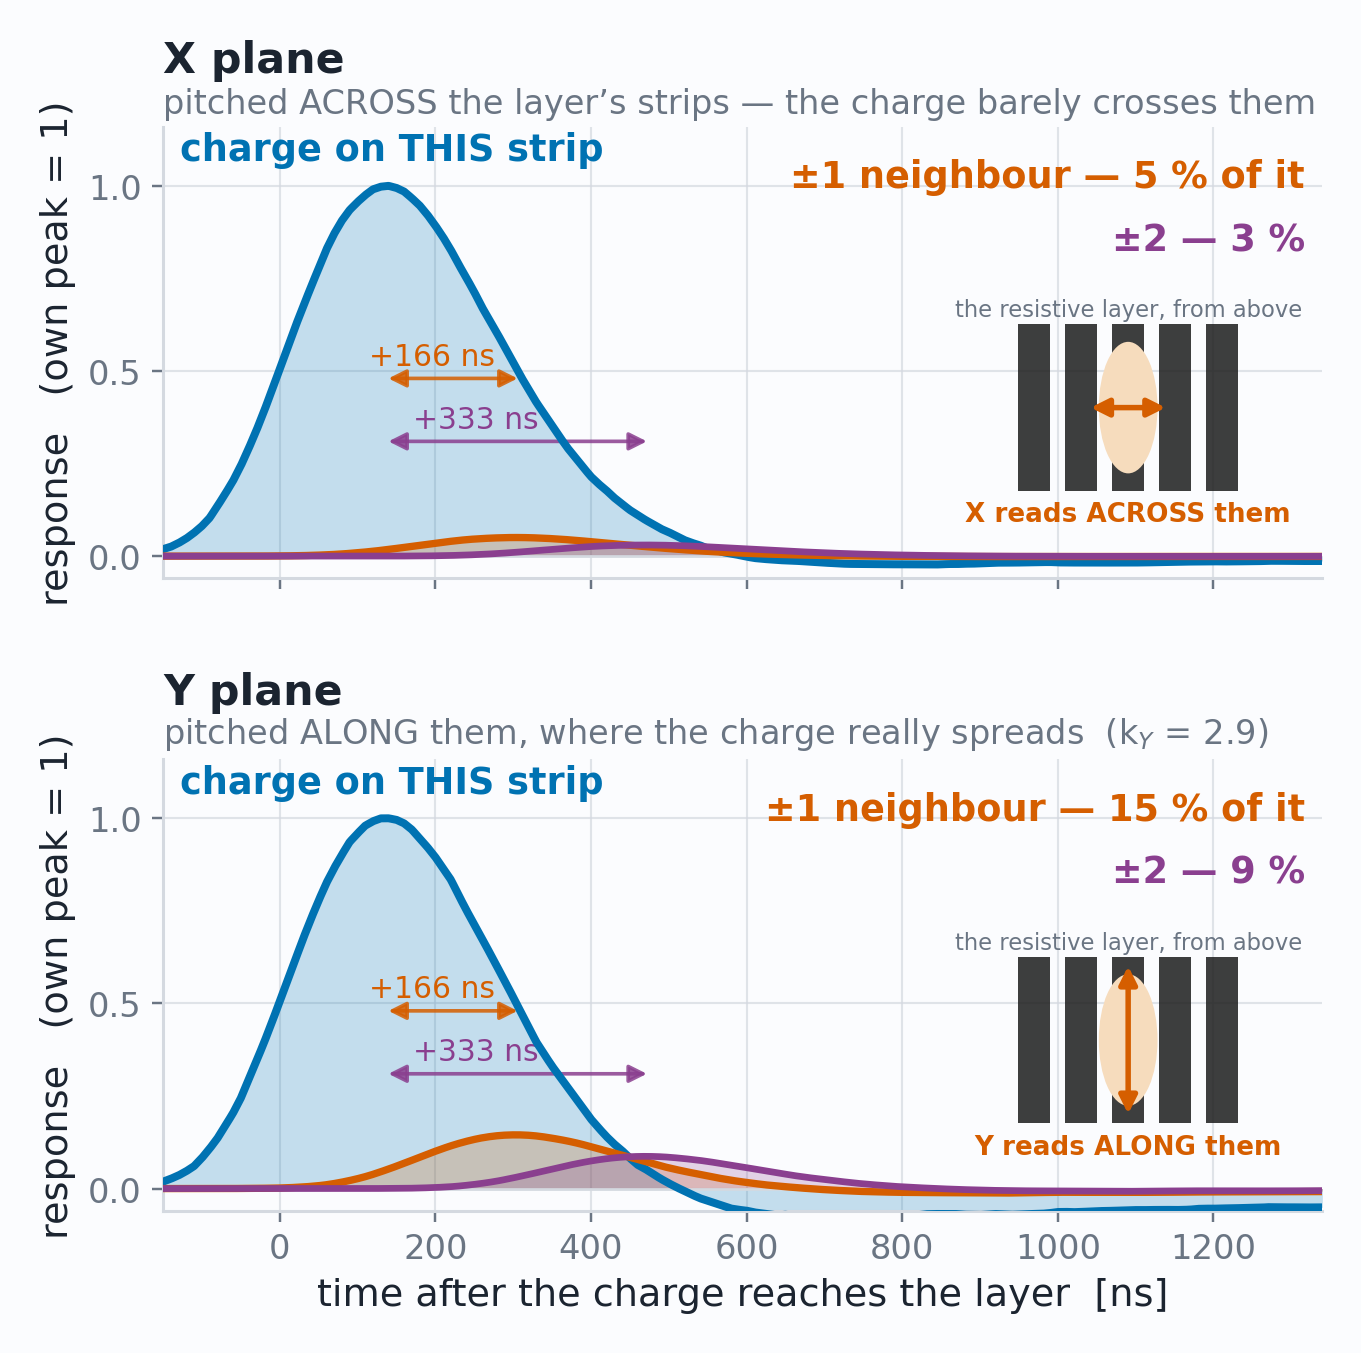
\includegraphics[width=0.50\textwidth]{figures/share_kernels.png}
\caption{\label{fig:detector} Left: one MX17 chamber, exploded along the drift axis (a
$44\times\SI{34}{mm^2}$ window at the real pitch). Right: measured response of a strip to charge
arriving on it (blue) and on its first and second neighbours (orange, purple), in the two views.
\askDylan{the rendered labels on these figures are small at this size: re-render larger for print?}}
\end{figure}

We therefore do not reconstruct from hit times. Following the T2K ND280 resistive-Micromegas
analysis~\cite{Attie2023}, a forward model predicts the waveform of every strip in the cluster
simultaneously: the track is parametrised by its arrival position and time at the mesh and its
transverse speed $w$; the charge in each drift-depth slice is solved by non-negative least squares;
each slice is folded through the strip geometry, the measured neighbour-sharing kernel and the
measured single-strip impulse response; and the track parameters minimise the $\chi^2$ against the
recorded waveforms (figure~\ref{fig:performance}, left). The drift velocity enters only at the end,
$\tan\theta = w/v_\text{drift}$. In contrast to charge-dispersion methods that use the neighbours to
refine a centroid, the fit returns the drift-depth charge profile, i.e.\ a $\mu$TPC segment free of
the neighbour-induced time bias.

%% ------------------------------------------------------------------------------------------
\section{Performance on cosmic rays and in a beam}
\label{sec:performance}

The chambers were characterised in June 2026 on the Saclay cosmic bench, in
Ar/iC$_4$H$_{10}$ (95/5) at a drift field of \SI{333}{V/cm}. Two chambers under test are
interleaved with four $50\times\SI{50}{cm^2}$ reference Micromegas, which provide a track with a
pointing resolution of about \SI{0.4}{mm} at the chamber; a coincidence of two
$60\times\SI{60}{cm^2}$ scintillators triggers the readout.

On the best chamber, 93.1\% of the \num{21953} reference muons are reconstructed within
\SI{5}{mm} of the reference track. Of the rest, 4.2\% are detected more than \SI{5}{mm} away (a
near-miss tail, mostly at large angles and close to the edges), 2.6\% coincide with a discharge in
the chamber and 0.2\% give a signal without a valid $x$--$y$ point; only 3 muons (0.01\%) produce no
signal at all. The efficiency is uniform over the active area. The other chambers range from 92\%
down to 42\%, the latter limited by regions of the amplification stage that never reach full gain.

The per-plane angular resolution, compared with the reference track and with the reference never
used in the fit, is $\sigma_{68} = \ang{1.19}$ ($x$) and \ang{1.23} ($y$) with a bias below
\ang{0.1} (figure~\ref{fig:performance}, right). Above $\sim\ang{5}$ it reaches $\approx\ang{1}$,
the limit set by diffusion and the granularity of the primary ionisation, so the per-event fit
extracts essentially all of the information the drift gap holds. Plane-to-plane timing is
\SI{33}{ns}, \SI{1.1}{mm} of drift. Since the bench resolution in position is dominated by the
reference tracks and multiple scattering, the spatial resolution was measured on one chamber in the
SPS H4 beam: \SI{176 \pm 35}{\micro m} at normal incidence, on the
chamber with the lowest gain of the set.

\begin{figure}[htbp]
\centering
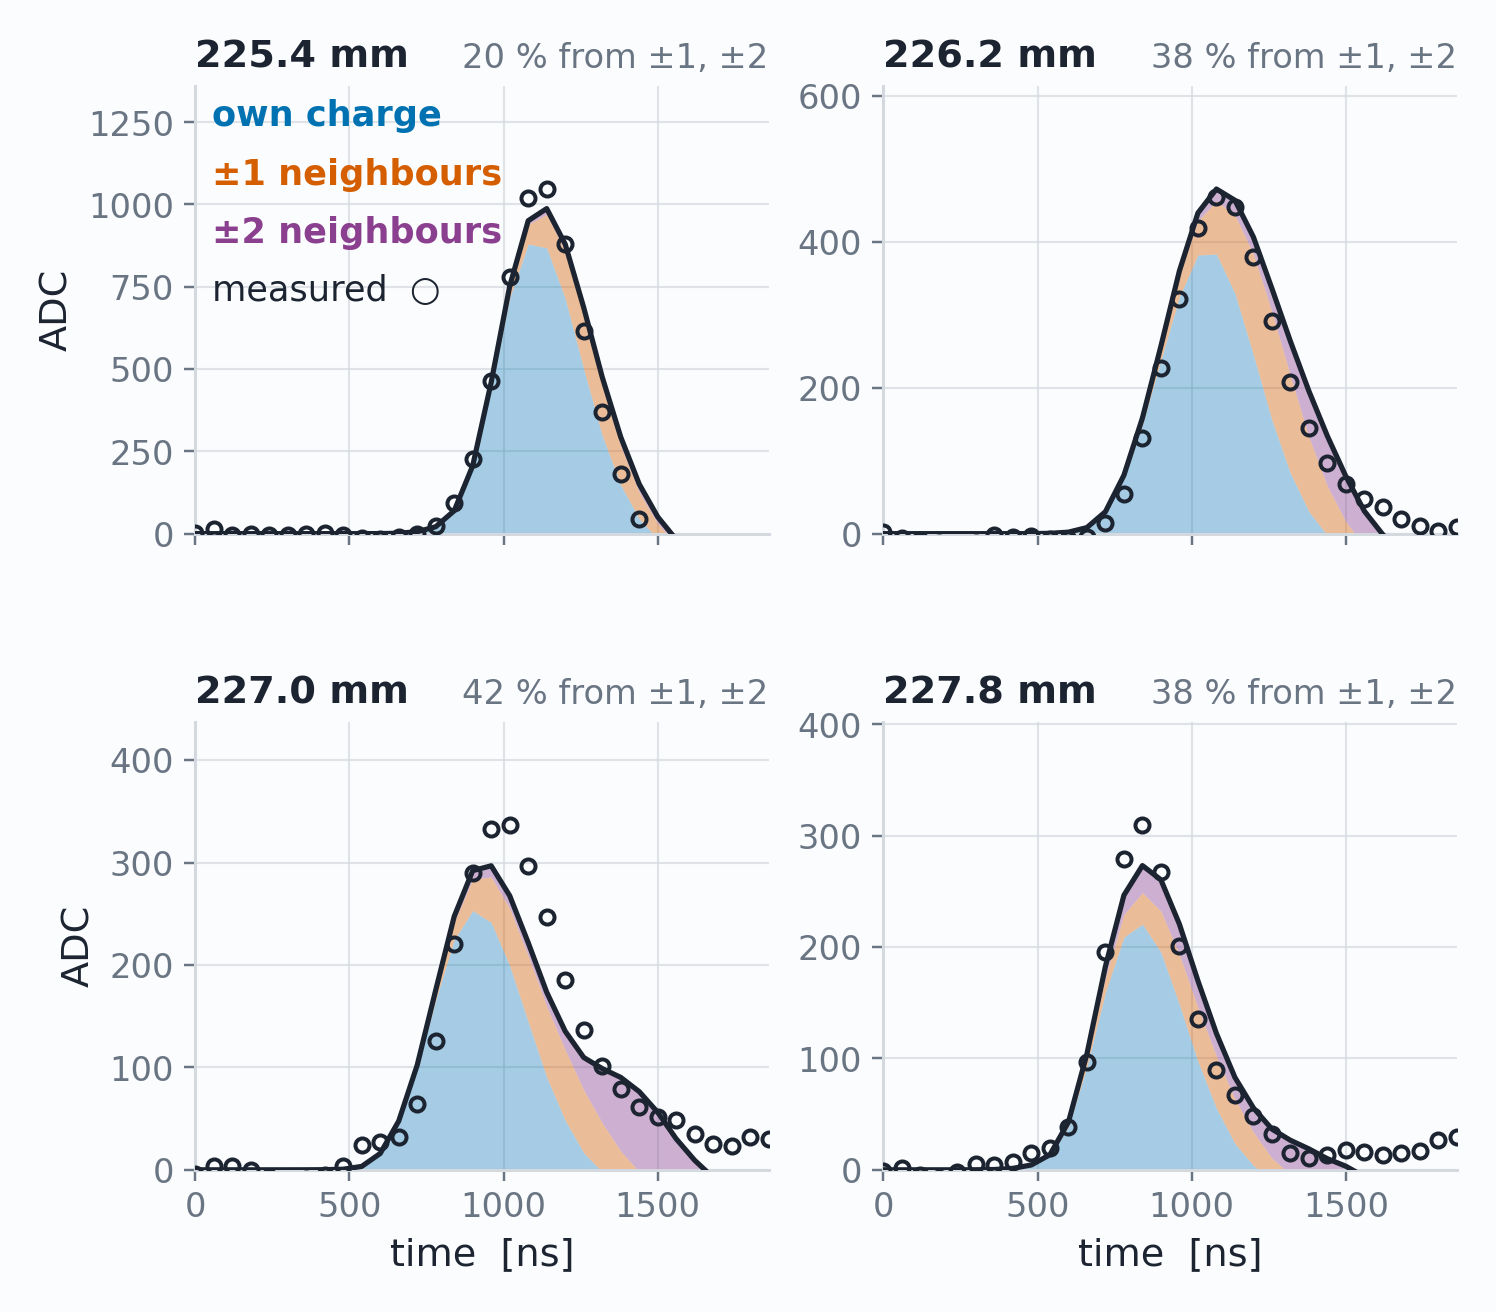
\includegraphics[width=0.46\textwidth]{figures/share_decompose.png}
\hfill
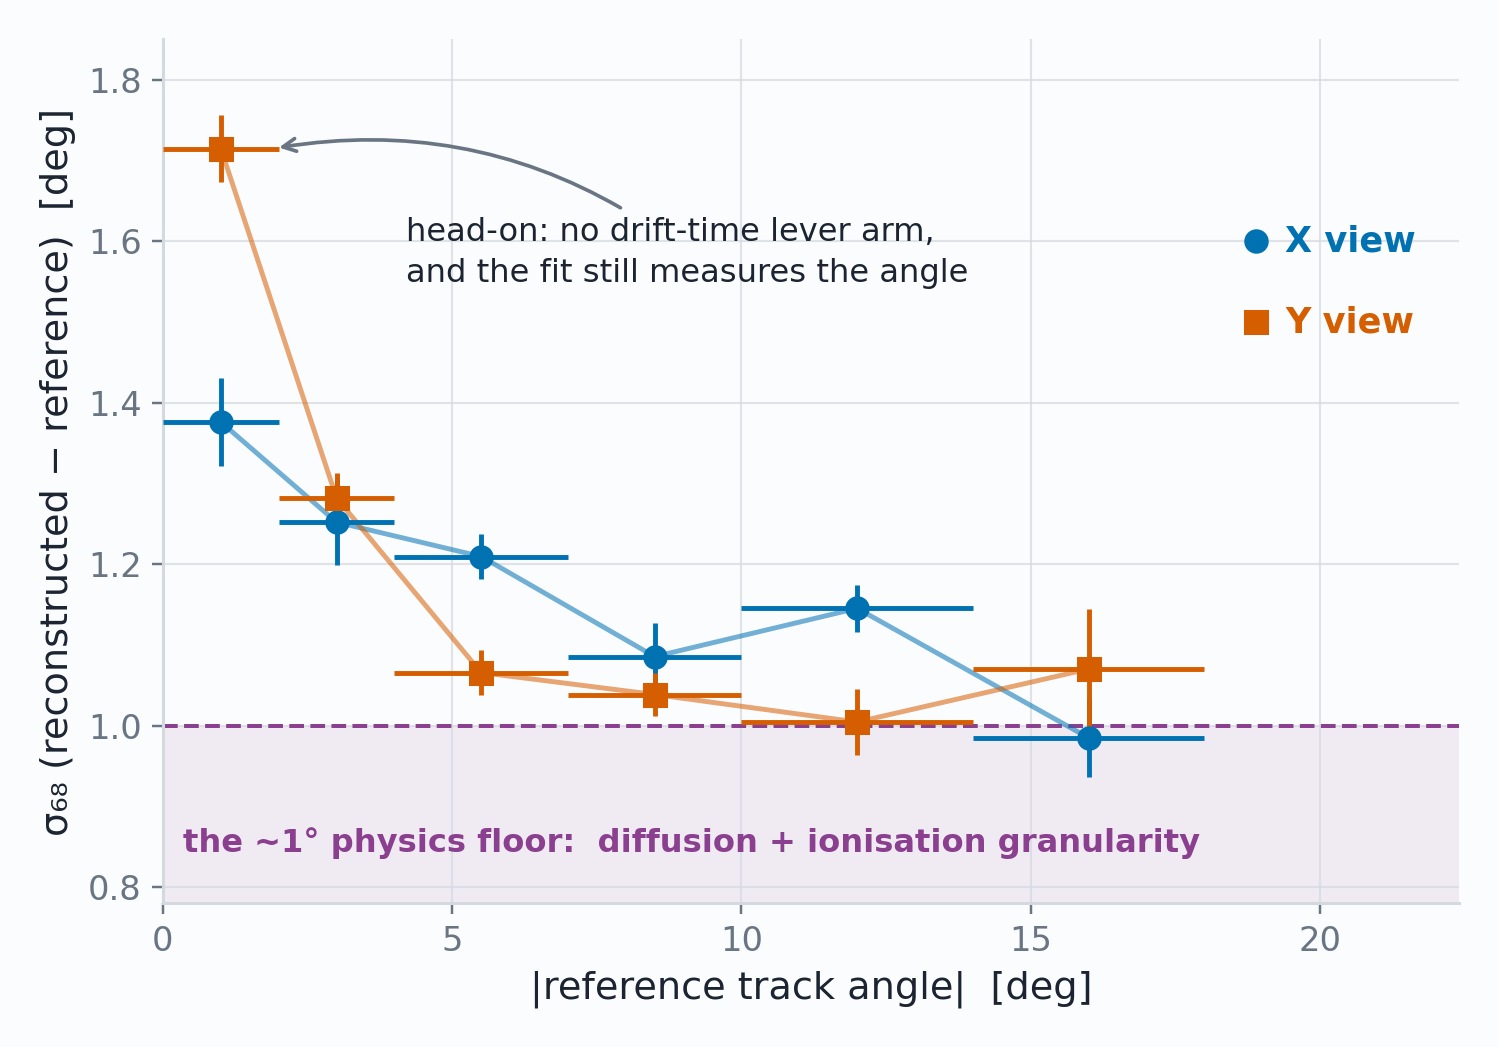
\includegraphics[width=0.50\textwidth]{figures/angle_resolution.png}
\caption{\label{fig:performance} Left: four consecutive strips of one cosmic muon (circles), with
the forward-model prediction decomposed into each strip's own charge and the charge shared from its
$\pm1$ and $\pm2$ neighbours. Right: per-plane angular resolution ($\sigma_{68}$ of reconstructed
minus reference angle) versus the angle of the reference track; the shaded band marks the
$\approx\ang{1}$ limit from diffusion and ionisation granularity.}
\end{figure}

%% ------------------------------------------------------------------------------------------
\section{The n\_TOF EAR2 measurement}
\label{sec:ntof}

At n\_TOF, \SI{20}{GeV/c} protons from the PS strike a lead spallation target; EAR2 sits about
\SI{20}{m} above it, at the end of a vertical flight path~\cite{Weiss2015}. The target is
\SI{500}{bar} of $^3$He in a capsule with a \SI{20}{mm} bore and \SI{40}{mm} of gas, with walls of
\SI{0.6}{mm} aluminium and a \SI{0.9}{mm} carbon-fibre overwrap. Four MX17 chambers face it in a
pinwheel, \SI{\approx 20}{cm} from the beam axis (figure~\ref{fig:setup}). Behind each chamber a wall
of thin scintillator bars read out by SiPMs and a \SI{2}{cm} plastic scintillator provide the
trigger (a coincidence within \SI{20}{ns}), followed by \SI{2}{cm} of liquid scintillator for
calorimetry. The opening angle is measured by the Micromegas before the pair reaches anything
else. The chambers were operated in Ar/iC$_4$H$_{10}$ (90/10) at a drift field of
\SI{233}{V/cm}.

\begin{figure}[htbp]
\centering
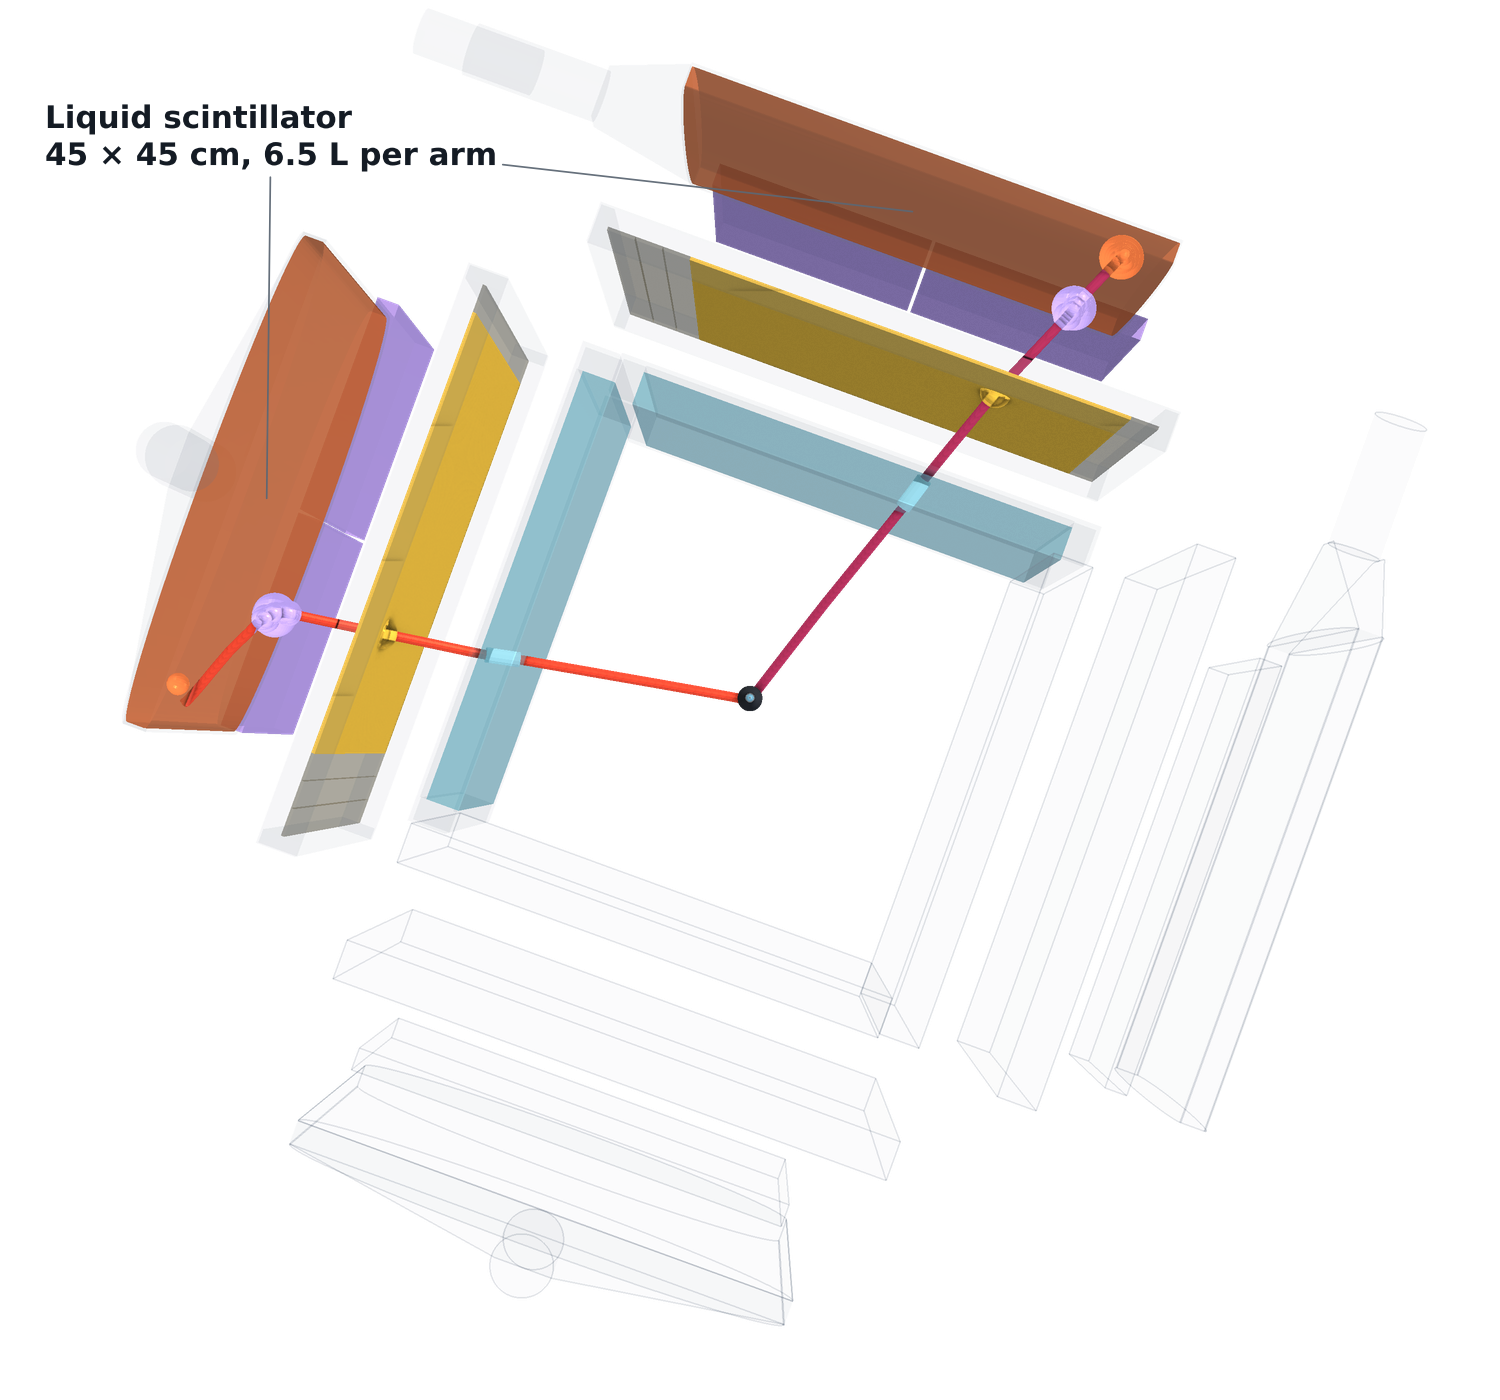
\includegraphics[width=0.50\textwidth]{figures/setup3d_9_full.png}
\qquad
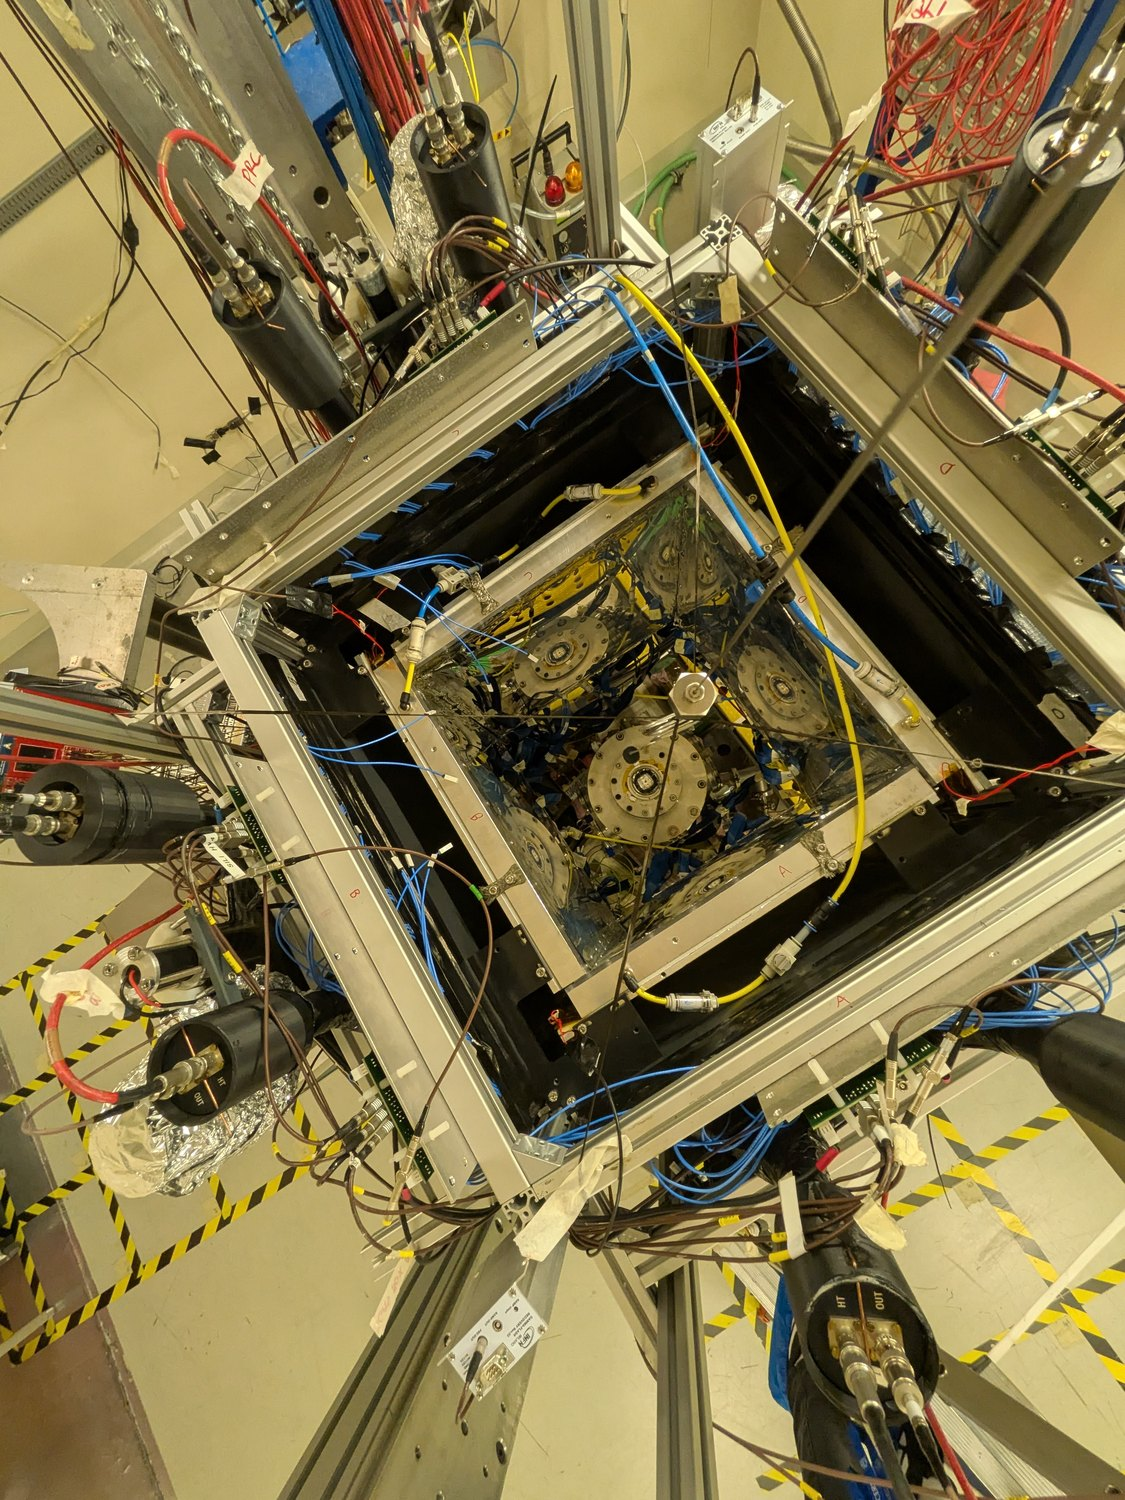
\includegraphics[width=0.33\textwidth]{figures/photo_station_topdown.jpg}
\caption{\label{fig:setup} Left: the measuring station (Geant4 geometry): the $^3$He capsule on the
vertical beam axis, surrounded by four Micromegas, the SiPM trigger walls and the plastic and liquid
scintillators. Right: the station in EAR2, viewed from above.}
\end{figure}

The physics run lasted from 28 June to 10 August 2026: \num{436373} proton pulses over 44 days,
with beam on target 78.6\% of the time. The DAQ recorded \num{41.8e6} events (\num{35.9e6} with beam,
\num{5.8e6} beam-off cosmic reference events), \SI{17.9}{TB} in total.

\paragraph{The $\gamma$ flash.} Each proton pulse produces an intense burst of photons and
relativistic particles, the $\gamma$ flash, which arrives before the neutrons. For neutron energies
in the MeV range, where the p-wave resonance enhances the X17 production~\cite{Viviani2022}, the
neutrons arrive between \SI{0.45}{\micro s} (\SI{10}{MeV}) and \SI{4.5}{\micro s} (\SI{0.1}{MeV})
after it. The flash deposits of order \SI{100}{nC} per chamber per pulse, estimated from the
mesh high-voltage current, and up to several hundred pC on a single strip, far beyond the
\SIrange{50}{600}{fC} full scale of the DREAM charge-sensitive amplifier. When the same chamber at
the same voltage (\SI{540}{V}) is digitised directly by the n\_TOF DAQ, without a charge amplifier,
its strip signal is back under threshold \SI{2.0}{\micro s} after the flash peak: the chamber
itself recovers within microseconds. Through DREAM, the front-end noise reappears only
\SI{5.0}{ms} after the flash, a factor $2.4\times10^3$ later (figure~\ref{fig:flash}). In the
first prototype test this saturation hid itself: the ADC rails, then settles onto a flat baseline
within \SI{\sim 3}{\micro s}, while the preamplifier is still pinned. The tell-tale sign is the
missing noise.

\begin{figure}[htbp]
\centering
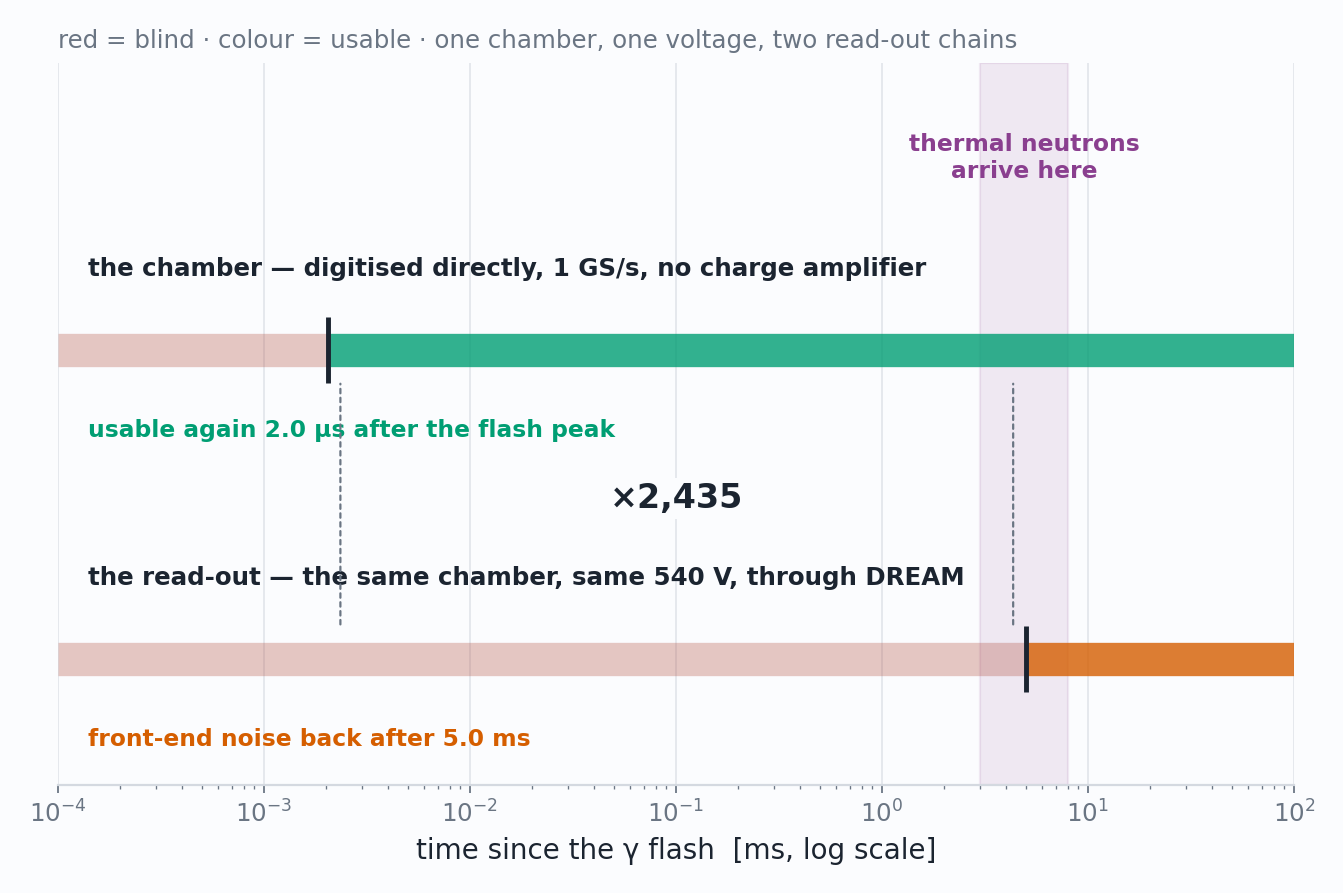
\includegraphics[width=0.62\textwidth]{figures/status_two_readouts_op.png}
\caption{\label{fig:flash} Time after the $\gamma$ flash at which the same chamber (detector A,
\SI{540}{V}) becomes usable again, digitised directly at \SI{1}{GS/s} without a charge amplifier
(top) and through the DREAM front end (bottom). Red: blind; colour: usable. The band marks the
arrival of thermal neutrons.}
\end{figure}

The front-end recovery time grows with the collected flash charge, and therefore with the
amplification voltage, while the detection efficiency falls as the voltage is lowered. The
operating point (\SI{540}{V}) was chosen from this trade-off, below the efficiency plateau of the
bench. With the MeV window out of reach, the trigger was opened from \SIrange{1}{30}{ms} after the
flash, which covers the thermal-neutron peak at \SI{5.3}{ms}. Below a few eV only the s-wave
capture channels remain open, so the IPC and any X17 contribution in these data have to be
interpreted with the thermal-capture physics, which differs from the MeV case.
\askDylan{Is this level of physics framing OK for the proceedings, or keep it purely to detector
operation? No absolute yields quoted on purpose (rate tables under review).}

\paragraph{First reconstructed tracks.} The bench reconstruction transfers to the beam data,
with the per-chamber calibration (drift velocity, angle scale) redone in situ. For a source on the
beam axis, a track crossing the strip plane at a distance $u$ from the beam-axis perpendicular must
arrive with $\tan\theta = u/L$, where $L\approx\SI{235}{mm}$ is the distance to the plane; the
reconstructed angles of tracks confirmed by the scintillators follow this relation. Projected back
to the target plane, tracks from two opposing chambers converge on the capsule
(figure~\ref{fig:pointing}). Both chambers independently place it \SI{\approx 9}{mm} off the nominal
beam axis, within its \SI{10}{mm} bore radius; the agreement between the two is at the level of
\SI{1}{mm}. These results are preliminary.

\begin{figure}[htbp]
\centering
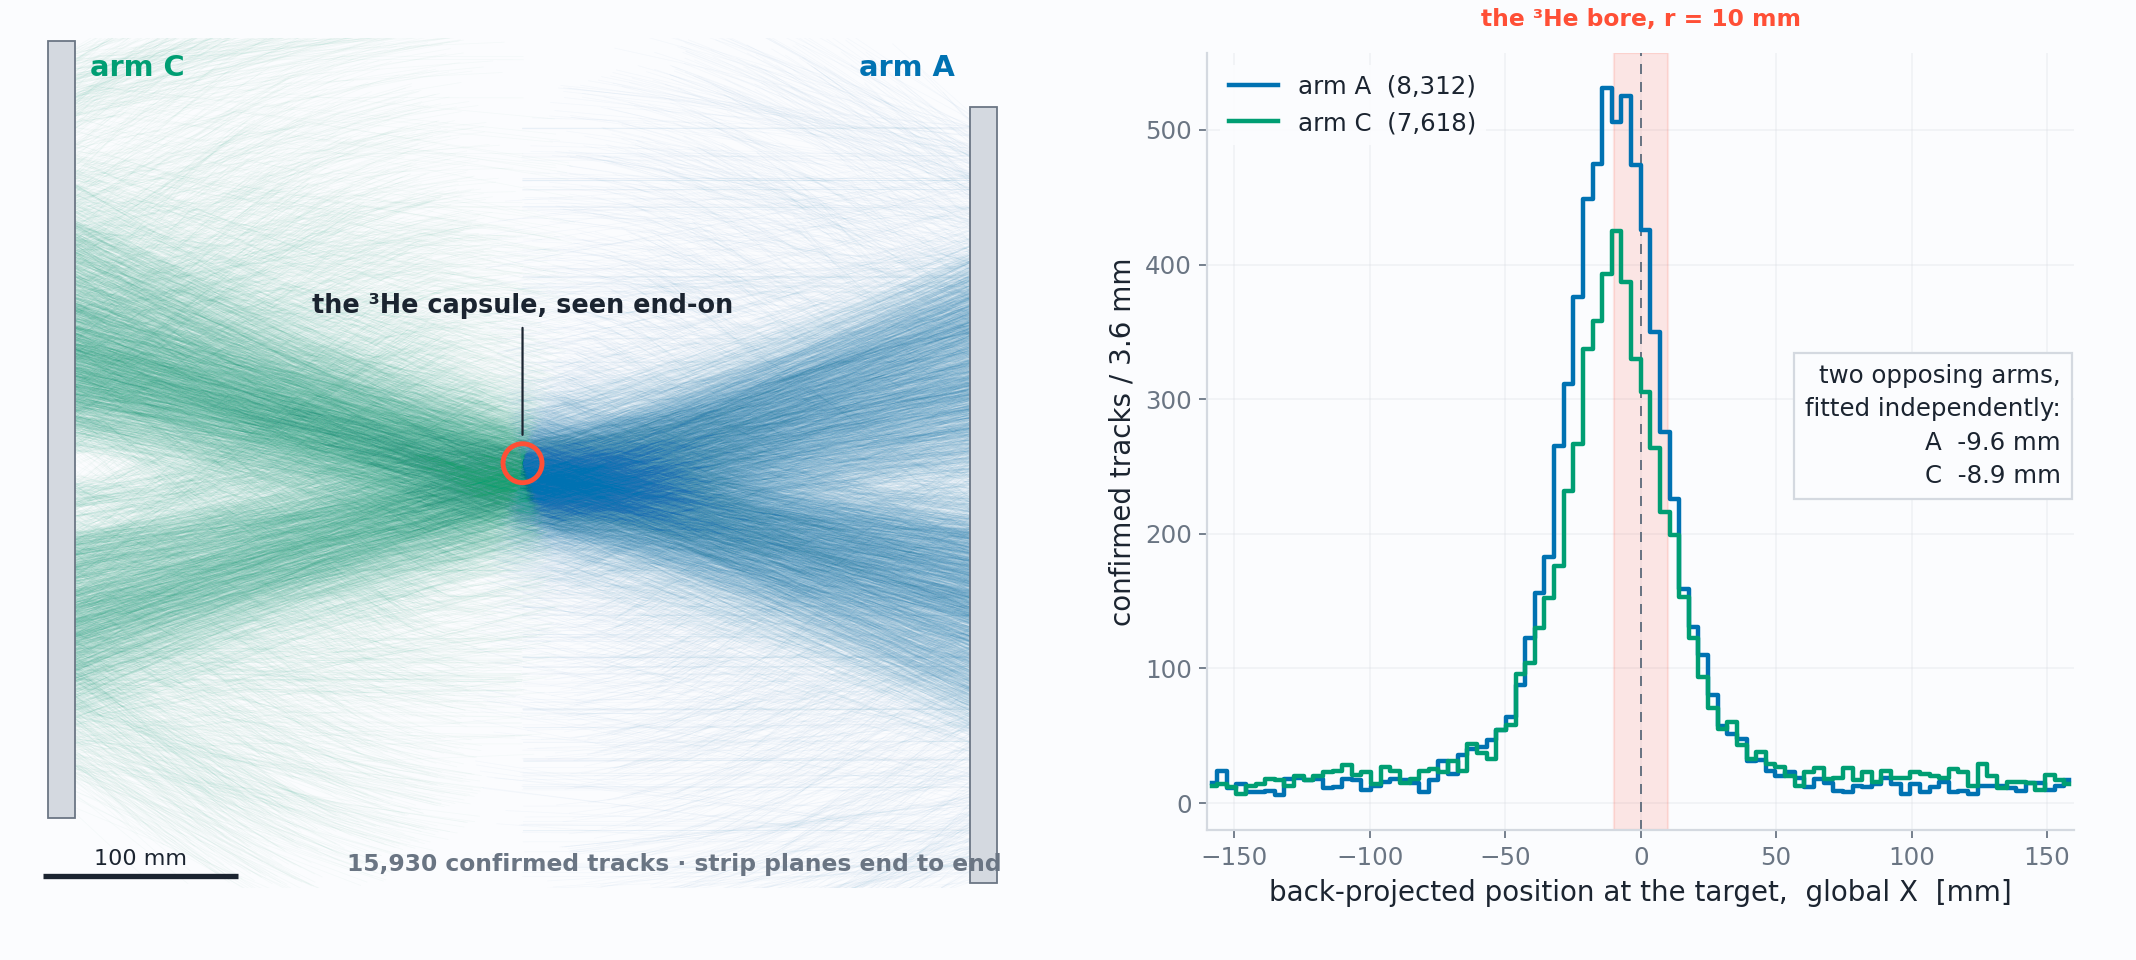
\includegraphics[width=0.80\textwidth]{figures/run145_overhead_AC.png}
\caption{\label{fig:pointing} Left: reconstructed tracks of two opposing chambers (A and C), seen
along the beam axis and extended from their strip planes to the beam axis. Right: back-projected
position at the target plane, for the two chambers fitted independently. Preliminary.}
\end{figure}

%% ------------------------------------------------------------------------------------------
\section{Summary and outlook}
\label{sec:summary}

Four $40\times\SI{40}{cm^2}$ resistive-strip Micromegas $\mu$TPCs were built and characterised for an
X17 search at n\_TOF. Because charge sharing on the resistive strips delays and disperses the
neighbouring signals, hit times are not a valid basis for $\mu$TPC reconstruction on these
detectors; a waveform forward model that includes the sharing reaches an angular resolution of
$\approx\ang{1.2}$, close to the physical limit of the drift gap, and 93\% efficiency on the best
chamber. The 2026 campaign at EAR2 is complete, with \num{41.8e6} events recorded. Its main
operational lesson concerns the electronics rather than the chambers: the $\gamma$ flash saturates
the charge-sensitive front end for milliseconds while the Micromegas recover within microseconds,
so a front end that tolerates the flash would open the MeV-neutron window. Tracks reconstructed in
the beam data point back to the target; the analysis now proceeds to two-track events and the
opening-angle spectrum.

%% ------------------------------------------------------------------------------------------
\acknowledgments

We thank the n\_TOF Collaboration, and especially the local team, for making the measurement
possible; S.~Aune and the CEA Saclay detector and electronics groups for building the detectors and
supplying the DAQ; the CERN EP-DT Gas Detector Development group and the CERN MPT workshop (bulk
production) for their support; and the MPGD2026 organisers. This work received funding from
EUROLABS. \askDylan{grant numbers (EUROLABS: Horizon Europe grant agreement No.~101057511?),
your own funding agency, and any names to add}

\begin{thebibliography}{99}

\bibitem{Krasznahorkay2016}
A.J.~Krasznahorkay et al., \emph{Observation of anomalous internal pair creation in $^8$Be: a
possible indication of a light, neutral boson}, \emph{Phys. Rev. Lett.} \textbf{116} (2016) 042501.

\bibitem{Krasznahorkay2021}
A.J.~Krasznahorkay et al., \emph{New anomaly observed in $^4$He supports the existence of the
hypothetical X17 particle}, \emph{Phys. Rev. C} \textbf{104} (2021) 044003.

\bibitem{Krasznahorkay2022}
A.J.~Krasznahorkay et al., \emph{New anomaly observed in $^{12}$C supports the existence and the
vector character of the hypothetical X17 boson}, \emph{Phys. Rev. C} \textbf{106} (2022) L061601.

\bibitem{Viviani2022}
M.~Viviani et al., \emph{X17 boson and the $^3$H$(p,e^+e^-)^4$He and $^3$He$(n,e^+e^-)^4$He
processes: a theoretical analysis}, \emph{Phys. Rev. C} \textbf{105} (2022) 014001.

\bibitem{Giomataris1996}
Y.~Giomataris, Ph.~Rebourgeard, J.P.~Robert and G.~Charpak, \emph{MICROMEGAS: a high-granularity
position-sensitive gaseous detector for high particle-flux environments}, \emph{Nucl. Instrum.
Meth. A} \textbf{376} (1996) 29.

\bibitem{Alexopoulos2011}
T.~Alexopoulos et al., \emph{A spark-resistant bulk-micromegas chamber for high-rate applications},
\emph{Nucl. Instrum. Meth. A} \textbf{640} (2011) 110.

\bibitem{DREAM}
\askDylan{DREAM ASIC reference, e.g.\ C.~Flouzat et al., \emph{Dream: a 64-channel front-end chip
with analogue trigger latency buffer for the Micromegas tracker of the CLAS12 experiment}, TWEPP
2014; or A.~Acker et al., \emph{The CLAS12 Micromegas Vertex Tracker}, Nucl. Instrum. Meth. A
\textbf{957} (2020) 163423 -- check}

\bibitem{Dixit2004}
M.S.~Dixit, J.~Dubeau, J.-P.~Martin and K.~Sachs, \emph{Position sensing from charge dispersion in
micro-pattern gas detectors with a resistive anode}, \emph{Nucl. Instrum. Meth. A} \textbf{518}
(2004) 721 [\href{https://arxiv.org/abs/physics/0307152}{\texttt{physics/0307152}}].

\bibitem{Galan2012}
J.~Galan et al., \emph{Signal propagation and spark mitigation in resistive strip read-outs},
\emph{2012 JINST} \textbf{7} C04009 [\href{https://arxiv.org/abs/1110.6640}{\texttt{arXiv:1110.6640}}].

\bibitem{Attie2023}
D.~Atti\'e et al., \emph{Characterization of charge spreading and gain of encapsulated resistive
Micromegas detectors for the upgrade of the T2K Near Detector Time Projection Chambers},
\emph{Nucl. Instrum. Meth. A} \textbf{1056} (2023) 168534
[\href{https://arxiv.org/abs/2303.04481}{\texttt{arXiv:2303.04481}}].

\bibitem{Weiss2015}
C.~Wei\ss{} et al., \emph{The new vertical neutron beam line at the CERN n\_TOF facility design and
outlook on the performance}, \emph{Nucl. Instrum. Meth. A} \textbf{799} (2015) 90.

\end{thebibliography}

\end{document}
